\documentclass[12pt, a4 paper]{article}
% Set target color model to RGB
\usepackage[inner=2.0cm,outer=2.0cm,top=2.5cm,bottom=2.5cm]{geometry}
\usepackage{setspace}
\usepackage[rgb]{xcolor}
\usepackage{environ}
\usepackage{verbatim}
\usepackage{subcaption}
\usepackage{outlines}
\usepackage{enumitem}
\usepackage{amsgen,amsmath,amstext,amsbsy,amsopn,tikz,amssymb,tkz-linknodes}
\usepackage{fancyhdr}
\usepackage{pgfplots}
\usepackage{mathtools}
\usepackage[colorlinks=true, urlcolor=blue,  linkcolor=blue, citecolor=blue]{hyperref}
\usepackage[colorinlistoftodos]{todonotes}
\usepackage{rotating}

\linespread{1.6} % Double Line Spacing
\usetikzlibrary{arrows.meta,intersections,calc}

\hypersetup{%
pdfauthor={Vignesh Ravibaskar},%
pdfcreator={PDFLaTeX},%
pdfproducer={PDFLaTeX},%
}

% Our custom enumerate labelling, just making the outlines bold basically
\setlist[enumerate,1]{label=\textbf{\arabic*}}
\setlist[enumerate,2]{label=\textbf{({\alph*})}}
\setlist[enumerate,3]{label=\textbf{({\roman*})}}

\title{Sequences \& Series}
\author{Derek, Vignesh}
\date{2020}

\newcommand{\comm}[1]{}
\NewEnviron{answer}{\vspace{3mm} \\ \color{blue} {\BODY} \color{black}}
% \NewEnviron{answer}{\color{blue} \comm{\BODY} \color{black}} % Use this method to hide all answers

\begin{document}

\maketitle

\textbf{SEQUENCES \& SERIES [80 Marks]}
\begin{outline}[enumerate]
\1 A geometric progression has first term \(a=\frac{1}{2}\) and common ratio \(r\). \(S_{n}\) denotes the sum of the first \(n\) terms of the progression. %Question 1

  \2 Given that the ratio \(S_{\infty}:a=3:2\), find $r$. \hfill[1]

  \2 Find the least value of \(k\) such that \(S_{k}\) is more than 99\% of \(S_{\infty}\).\hfill[3]

\1 The sum of the first \(n\) terms of a series is given by \(S_{n}=12-12\left(\frac{5}{6}\right)^{n}\). %Question 2

  \2 Find \(u_{n}\). Hence, show that the series is geometric. \hfill[2]

  \2 It is given that \(u_{1}\) and \(u_{2}\) are the third and fourth term respectively of an arithmetic progression \(v_{1},v_{2},\dots\). Find \(v_{n}\) in terms of \(n\).\hfill[3]

\1 A wire artist has a piece of wire of length \(L\). With one piece of wire, he can choose to make a different number of circles of different radiuses as shown: %Question 3
\[
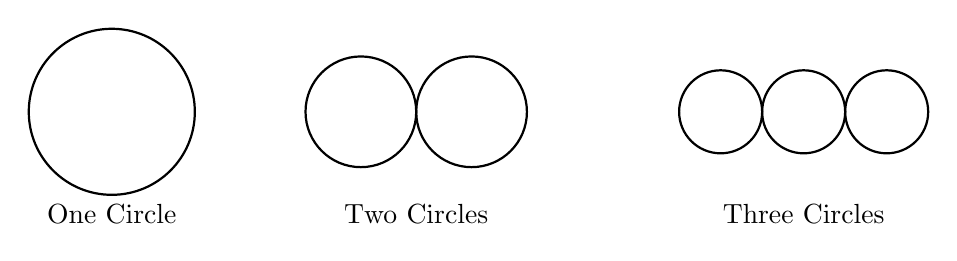
\begin{tikzpicture}
  \draw[thick] (0,0) circle (30pt);
  \draw (0,-30pt) node[below]{One Circle};
  \draw[thick] (90pt,0) circle (20pt);
  \draw[thick] (130pt,0) circle (20pt);
  \draw (110pt,-30pt) node[below]{Two Circles};
  \draw[thick] (220pt,0) circle (15pt);
  \draw[thick] (250pt,0) circle (15pt);
  \draw[thick] (280pt,0) circle (15pt);
  \draw (250pt,-30pt) node[below]{Three Circles};
\end{tikzpicture}
\]
  \2 Show that the area of the circles \(A_{n}\), where \(n\) denotes the number of circles formed with the wire, does not follow a geometric progression.\hfill[3]

  \2 It is given that \(B=\frac{1}{A}\). Describe the progression \(B_{1},B_{2},\dots,B_{n},\dots\).\hfill[2]

\1 Equilateral triangle \(ABC\) is inscribed in circle \(ABC\) of radius \(r\) as shown in the diagram below. A circle is then inscribed in \(\Delta ABC\), and the process continues indefinitely. %Question 4
\[
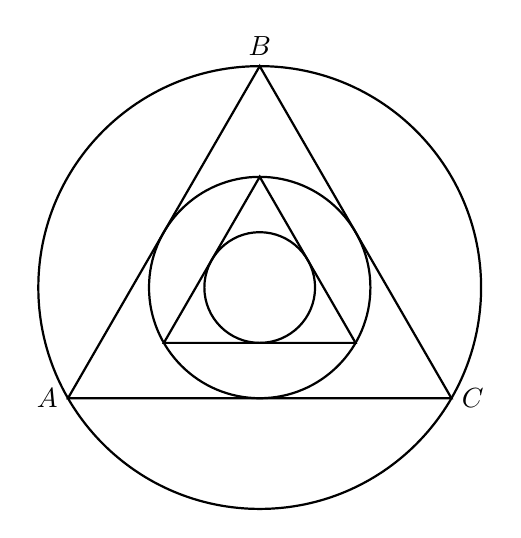
\begin{tikzpicture}
  \draw[thick] (0,0) circle (80pt);
  \draw[thick] (0,80pt) node[above]{\(B\)} -- (69.282pt,-40pt) node[right]{\(C\)} -- (-69.282pt,-40pt) node[left]{\(A\)} -- cycle;
  \draw[thick] (0,0) circle (40pt);
  \draw[thick] (0,40pt) -- (34.641pt,-20pt) -- (-34.641pt,-20pt) -- cycle;
  \draw[thick] (0,0) circle (20pt);
\end{tikzpicture}
\]
  \2 Show that the areas of the equilateral triangles form a geometric progression. Hence, state the sum to infinity of this geometric progression. \hfill[5]

  \2 An architect uses a similar design to build the tallest structure in the world constructed by cuboids stacked on top of cylinders stacked on top of cuboids and so on. Each cylindrical block is 20 storeys high and each cuboid block is 10 storeys high, where each storey is 3 metres in height. The first block, a cylinder, has a radius of 100 metres. Below is the bird's eye view of the building:
  \[
  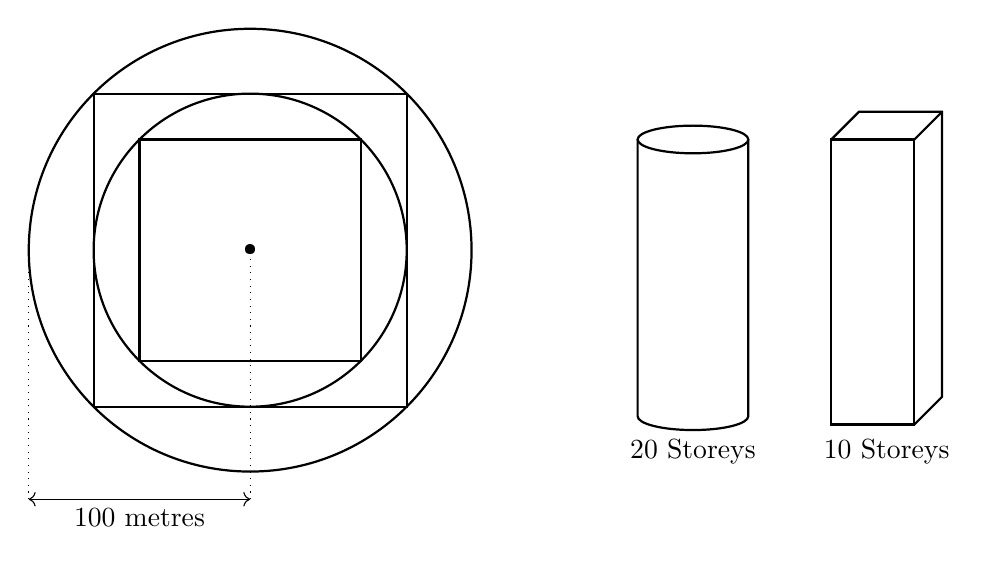
\begin{tikzpicture}
    \draw[<->] (-80pt,-90pt) -- (-40pt,-90pt)node[below]{100 metres} -- (0,-90pt);
    \draw[dotted] (-80pt,-90pt) -- (-80pt,0);
    \draw[dotted] (0pt,-90pt) -- (0,0);
    \draw[thick] (0,0) circle (80pt);
    \draw[thick] (56.5685pt,56.5685pt) -- (-56.5685pt,56.5685pt) --(-56.5685pt,-56.5685pt) -- (56.5685pt,-56.5685pt) -- cycle;
    \draw[thick] (0,0) circle (56.5685pt);
    \draw[thick] (40pt,40pt) -- (-40pt,40pt) --(-40pt,-40pt) -- (40pt,-40pt) -- cycle;
    \draw[thick] (160pt,40pt) ellipse (20pt and 5pt);
    \draw[thick] (140pt,40pt) -- (140pt,-60pt) arc (180:360:20pt and 5pt) -- (180pt,40pt);
    \draw[thick] (210pt,40pt) rectangle (240pt,-63pt);
    \draw[thick] (210pt,40pt) -- (220pt,50pt) -- (250pt,50pt) -- (250pt,-53pt) -- (240pt,-63pt);
    \draw[thick] (250pt,50pt) -- (240pt,40pt);
    \draw (160pt,-65pt) node[below]{20 Storeys};
    \draw (230pt,-65pt) node[below]{10 Storeys};
    \node at (0,0) {\textbullet};
  \end{tikzpicture}
  \]
  Due to building restrictions, the area of a block must be at least 60 m\(^2\). Find the maximum height the building can be built to.\hfill[5]

\1 On 1 January 2020, Jill has \$100,000 in her bank account. According to her savings plan, 2\% of her savings will be credited to this same account at the end of each month. %Question 5

  \2 Given that she spends \$5000 at the start of every month including January, find the least value of \(n\) such that she cannot finance her expenses in the \(n\)th month.\hfill[3]

  \2 Given instead that Jill spends \$\(k\) at the start of every month including January, find the greatest value of \$\(k\) such that she can afford a \$25,000 car at the end of 2020. \hfill[4]

\1 On 1 January 2020, Jack has \$5,000 in his bank account. He is looking for a savings plan to maximise his savings. Given that he spends \$200 at the start of every month including January, what is the minimum value of \(r\), where \(r\)\% is the interest rate under the savings plan, such that Jack's balance will not go below \$4,000 by the end of 2020? \hfill[5]

\end{outline}

\end{document}
